% SPDX-License-Identifier: LPPL-1.3c
% Copyright (C) 2026 Christophe Jorssen
% Author and Current Maintainer: Christophe Jorssen <christophe.jorssen@gmail.com>
% LPPL maintenance status: maintained
% This file is part of luafemm. See LICENSE and LICENSES.md for its terms.
\documentclass[a4paper,11pt]{article}
\usepackage[margin=17mm]{geometry}
\usepackage{fontspec}
\usepackage{luafemm}
\usepackage{pgfplots}
\pgfplotsset{compat=1.18}
\pagestyle{empty}
\begin{document}
\noindent{\Large\bfseries FEMM materials and field profiles}\par
\smallskip
\noindent\textsf{luafemm \luafemmversion{} · Lua computation · PGFPlots graphs}

\smallskip
\noindent The U and armature use \texttt{pure-iron}; the crosspiece uses
\texttt{cast-alnico-5-lng37}. The side rectangle uses \texttt{copper}.
All four materials, including air, come from the FEMM library.
No current is imposed.

\begin{center}
\begin{tikzpicture}[femm/problem={xmin=-90,xmax=90,ymin=-70,ymax=85,mesh size=3}]
  \filldraw[femm/region={material=pure-iron},fill=gray!15]
    (-40,-30)--(40,-30)--(40,30)--(25,30)--(25,-15)
    --(-25,-15)--(-25,30)--(-40,30)--cycle;
  \filldraw[femm/region={material=cast-alnico-5-lng37,magnetization angle=180},
    fill=red!25] (-25,-30) rectangle (25,-15);
  \filldraw[femm/region={material=pure-iron},fill=gray!15]
    (-40,31) rectangle (40,46);
  \filldraw[femm/region={material=copper},fill=orange!30]
    (49,-15) rectangle (56,15);
  \path[femm/region={material=air,mesh size=.5}]
    (-40,30) rectangle (-25,31);
  \path[femm/region={material=air,mesh size=.5}]
    (25,30) rectangle (40,31);
  \begin{scope}
    \clip (-57,-38) rectangle (62,52);
    \pic[femm/lines=19,femm/field style={teal!70!black}] {femm field};
  \end{scope}
  \draw[femm/profile={name=gap,samples=301},orange!85!black,dashed,thick]
    (-48,30.5)--(48,30.5) node[right,font=\small] {profile 1};
  \draw[femm/profile={name=curve,samples=201,curve tolerance=.01},
    violet,dashed,thick,-Stealth]
    (-18,-8) .. controls (-22,22) and (22,22) .. (18,-8);
  \node[violet,font=\small] at (0,6) {profile 2};
  \node[fill=red!25,font=\small] at (0,-22.5) {Alnico 5};
  \node[fill=gray!15,font=\small] at (0,39) {Soft iron};
  \node[rotate=90,font=\small] at (52.5,0) {Cu};
\end{tikzpicture}

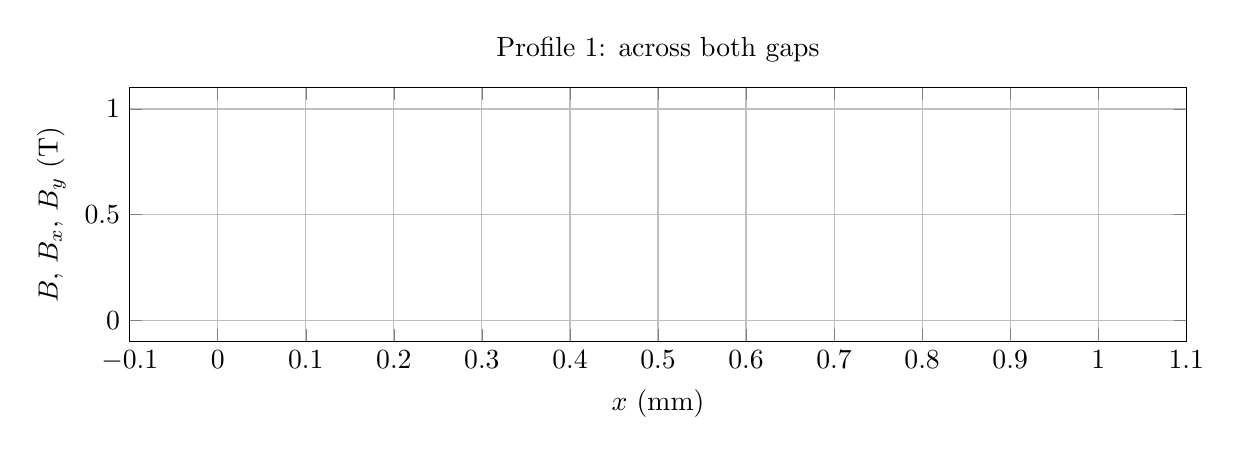
\begin{tikzpicture}
\begin{axis}[width=15cm,height=4.8cm,grid=major,
  xlabel={$x$ (mm)},ylabel={$B$, $B_x$, $B_y$ (T)},
  title={Profile 1: across both gaps},
  legend style={at={(1.02,1)},anchor=north west},no markers]
  \femmplot[profile=gap,component=B,abscissa=x,plot options={black,thick}]
  \addlegendentry{$|\mathbf B|$}
  \femmplot[profile=gap,component=Bx,abscissa=x,plot options={blue}]
  \addlegendentry{$B_x$}
  \femmplot[profile=gap,component=By,abscissa=x,plot options={red}]
  \addlegendentry{$B_y$}
\end{axis}
\end{tikzpicture}

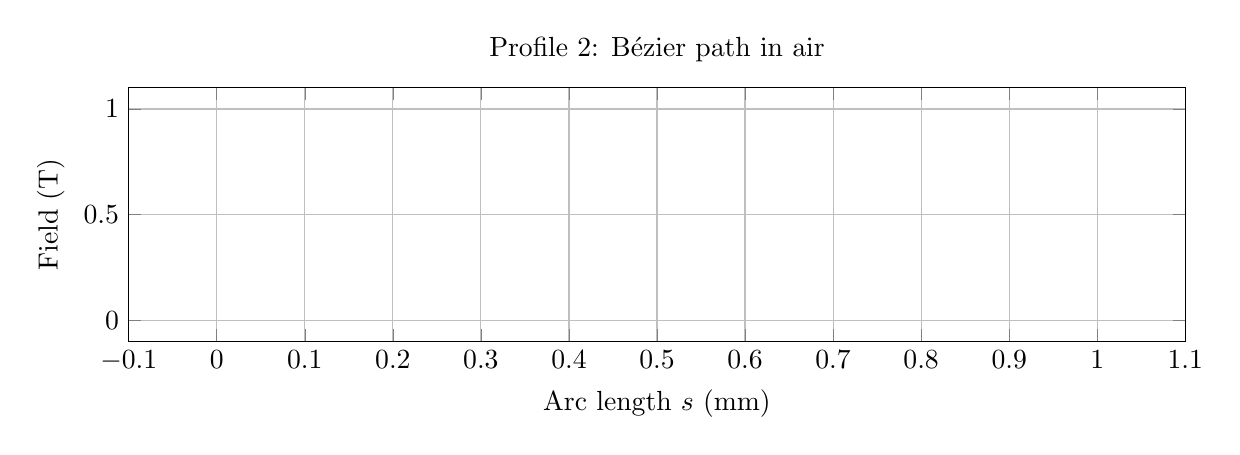
\begin{tikzpicture}
\begin{axis}[width=15cm,height=4.8cm,grid=major,
  xlabel={Arc length $s$ (mm)},ylabel={Field (T)},
  title={Profile 2: B\'ezier path in air},
  legend style={at={(1.02,1)},anchor=north west},no markers]
  \femmplot[profile=curve,component=B,plot options={black,thick}]
  \addlegendentry{$|\mathbf B|$}
  \femmplot[profile=curve,component=Bt,plot options={violet}]
  \addlegendentry{$B_t$}
  \femmplot[profile=curve,component=Bn,plot options={teal!70!black}]
  \addlegendentry{$B_n$}
\end{axis}
\end{tikzpicture}
\end{center}
\noindent\small Samples are equally spaced along the flattened path.
The $P_1$ fields are constant in each triangle; their small jumps are
preserved. The normal points to the left of the traversal direction.
The library retains FEMM properties; the computation uses planar magnetostatics.
\end{document}
